\chapter{Experiments}
\label{experiments_chapter}
In this chapter, we will evaluate the performance of the various agents when
confronted with different combinations of obstacles, as well as presenting interesting observations made during the experiments. One of the key questions we aim to answer is whether any of the agents are a are capable of learning to play the entire game. To begin, it is important to explain how the experiments were conducted and the significance of the plots in the following subsections of this chapter.

\section{Conducting the experiments}
The process of conducting experiments encountered several challenges and fluctuations. Initially, the primary concern was to determine the appropriate number of rotations (\texttt{rots}) and distances (\texttt{dists}) for each obstacle type (explained in Table \ref{commOpt}). After experimenting with up to 30 rotations in some cases, and not getting satisfying results with seemingly any combination of other parameters, it was determined that the game's difficulty in later levels was the root of the problem, as confirmed by human players. Consequently, the game had to be adjusted and thus, there are slight variations in parameters, such as the starting speed and distances between obstacles, in the version of the ``Space-run'' game used in this thesis, as compared to the original. As per a human player's assessment, it is now possible to play all environment combinations until level 15 or even beyond. It is noteworthy that level 10 was the initial choice for the winning level, which was later shifted to level 15 to prevent the agent from settling for a mediocre policy and to find the optimal policy. However, this shift did not yield significant results, and the same behaviour could likely be achieved by increasing the number of games, allowing the $\epsilon$-greedy policy to perform random moves more frequently for an extended period. Despite this, level 15 was used in all subsequent experiments.

\begin{figure}[h]
    \centering
    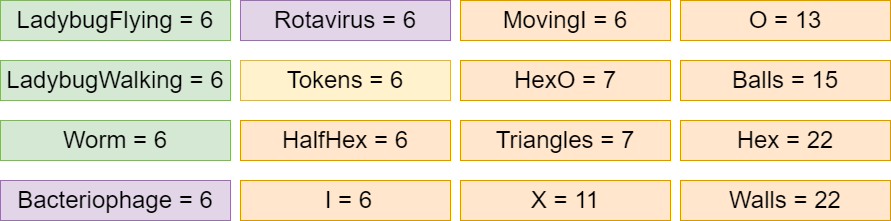
\includegraphics[width=\textwidth]{rot_values}
    \caption{\texttt{rots} values used for each obstacle type}
    \label{fig:rot_values}
\end{figure}

After addressing the the issue of game not being playable, the most straightforward method for identifying the number of rotations required was to play the game manually in debug mode. The results obtained from these experiments are displayed in Figure \ref{fig:rot_values} and were used in all experiments conducted. However, for obstacles such as \texttt{Walls} and \texttt{Balls}, this method was not viable. The reason being that running \texttt{env=Balls} or \texttt{env=Walls} with visuals caused the game to lag significantly due to the number of animations playing simultaneously. As a result, \texttt{Walls} received the same number of rotations as \texttt{Hex} trap, while \texttt{Balls} received 15 rotations, the number at which the agent managed to learn. For bug, virus, and token obstacles, the default and minimum value of 6 rotations was assigned, with which they all trained successfully.
Concerning the \texttt{dists} parameter, it was concluded during the experiments that all agents could learn any obstacle with \texttt{dists=1}, and increasing this number needlessly would only increase the number of states required for training. 

The remaining values to be determined for the experiments were the suboptions for each agent (see \ref{opt:agent}).  The reader must realize that there were a lot of experiments conducted that had to be disregarded later on for this or that reason, but they provided useful insights that could be utilized. For instance, in many of those experiments, the agent performed best with \texttt{eps} values ranging from 0.2 to 0.4, with 0.2 being the most common, in combination with an \texttt{epsFinal} value of 0.0001. The rationale for using a low \texttt{epsFinal} value is that towards the end, the agent almost exclusively exploits the current policy, and a more gradual decrease in epsilon values is suitable for larger values of \texttt{n}. Furthermore, \texttt{initOptVal} of 20.0 and 100.0 was promising in most experiments. The \texttt{gam} value will be discussed in a later subsection.

Throughout the months dedicated to conducting experiments, they gradually converged towards checking combinations of the values mentioned above. In some instances, other values were experimented with and will be discussed when exploring various environments in later subsections. However, due to the length of the experiments and the number of parameters requiring adjustment, they were kept systematic towards the end, and most of the results presented in this chapter were obtained from experiments run with different \texttt{env} and value \texttt{n} adjusted according to the environment. Each combination was tested on ten seeds for each agent, with the combinations consisting of \texttt{eps} parameter taking a value of either 0.2 or 0.4, and the \texttt{initOptVal} being either 20.0 or 100.0. Discounting was kept at the value of 1 and \texttt{epsFinal} was 0.0001.

\section{Plotting}
\section{Interesting behaviours}
\section{Individual traps environment}
\section{Traps environment}
\section{Tokens environment}
\section{Bugs environment}
\section{Viruses environment}
\section{Full game environment}